\documentclass[a4paper,14pt]{extreport} %размер бумаги устанавливаем А4, шрифт 12пунктов
\usepackage[T2A]{fontenc}
\usepackage[utf8]{inputenc}%включаем свою кодировку: koi8-r или utf8 в UNIX, cp1251 в 
\usepackage[english,russian]{babel}
\usepackage{amssymb,amsfonts,amsmath,mathtext,cite,enumerate,float}
\usepackage{hyperref}
\renewcommand{\rmdefault}{ftm}

\usepackage{geometry}
\geometry{left=3cm}
\geometry{right=1.5cm}
\geometry{top=2.0cm}
\geometry{bottom=2.0cm}

\renewcommand{\baselinestretch}{1.3}  % 1 интервал

\renewcommand{\thetable}{\arabic{section}.\arabic{table}}

%\renewcommand{\captionlabeldelim}{ \textendash}

\tolerance=10000

\newcommand{\D}{\mathrm{d}}
% Производные
\newcommand{\dsl}[2]{{\partial #1}/{\partial #2}}
\newcommand{\df}[1]{\cfrac{\partial}{\partial #1}}
\newcommand{\dff}[2]{\frac{\partial #1}{\partial #2}}
\newcommand{\dfs}[2]{\frac{\partial^2 #1}{\partial #2^2}}
\newcommand{\dfss}[3]{\frac{\partial^2 #1}{\partial #2\, \partial #3}}
\newcommand{\Df}[1]{\frac{d}{d #1}}
\newcommand{\Dff}[2]{\frac{d #1}{d #2}}
\newcommand{\Dfs}[2]{\frac{d^2 #1}{d #2^2}}
\newcommand{\cDf}[1]{\cfrac{d}{d #1}}
\newcommand{\cDff}[2]{\cfrac{d #1}{d #2}}
\newcommand{\cDfs}[2]{\cfrac{d^2 #1}{d #2^2}}
\newcommand{\dfn}[3]{\frac{\partial^#1 #2}{\partial #3^#1}}
% Векторы
\renewcommand{\vec}[1]{\bm{#1}}
\newcommand{\ort}[1]{\bm{\mathrm{e}}_#1}
% Векторный анализ
\renewcommand{\div}{\mathrm{div}\,}
\newcommand{\rot}{\mathrm{rot}\,}
\newcommand{\grad}{\mathrm{grad}\,}
\newcommand{\laplas}[4]{\dfs{#1}{#2}+\dfs{#1}{#3}+\dfs{#1}{#4}}
\newcommand{\laplasxyz}[1]{\dfs{#1}{x}+\dfs{#1}{y}+\dfs{#1}{z}}
\newcommand{\rotc}[4]{\dff{#1}{#2} - \dff{#3}{#4}}
\newcommand{\rotcx}[3]{\dff{#1\vphantom{E}_#3}{#2} - \dff{#1\vphantom{E}_#2}{#3}}
% Функции
\renewcommand{\cosh}{\mathrm{ch}\,}
\renewcommand{\sinh}{\mathrm{sh}\,}
\renewcommand{\tanh}{\mathrm{th}\,}
\renewcommand{\Im}{\mathrm{Im}\,}
\renewcommand{\Re}{\mathrm{Re}\,}
\renewcommand{\det}[4]{#1 #4 - #2 #3}
\renewcommand{\matrix}[4]{\begin{pmatrix}#1 & #2 \\ #3 & #4\end{pmatrix}}
\newcommand{\matrixw}[5]{\begin{#5matrix}#1 & #2 \\ #3 & #4\end{#5matrix}} % #5 = b p s v V
\newcommand{\col}[2]{\begin{pmatrix}#1 & #2\end{pmatrix}}
\newcommand{\colw}[3]{\begin{#3matrix}#1 & #2 \end{#3matrix}} % #3 = b p s v V
\newcommand{\row}[2]{\begin{pmatrix}#1 \\ #2\end{pmatrix}}
\newcommand{\roww}[3]{\begin{#3matrix}#1 \\ #2 \end{#3matrix}} % #3 = b p s v V
\newcommand{\matrixt}[2]{\begin{#1matrix} #2\end{#1matrix}}
\newcommand{\matrixrotr}[7]{\begin{#1matrix} \ort{#2} & \ort{#3} & \ort{#4} \\ \df{#2} & \df{#3} & \df{#4} \\ #5 & #6 & #7 \end{#1matrix}}
\newcommand{\matrixrotd}[4]{\begin{#1matrix} \ort{x} & \ort{y} & \ort{z} \\ \df{x} & \df{y} & \df{z} \\ #2 & #3 & #4 \end{#1matrix}}
\newcommand{\matrixrotdv}[2]{\begin{#1matrix} \ort{x} & \ort{y} & \ort{z} \\ \df{x} & \df{y} & \df{z} \\ #2_x & #2_y & #2_z \end{#1matrix}}
\newcommand{\eps}{\varepsilon}
\renewcommand{\phi}{\varphi}

\newcommand{\shtr}{\mathop{\!\vphantom{E}'}}
\newcommand{\ind}[1]{\mathop{\!\vphantom{E}_{#1}}}
%\renewcommand{\theequation}{\arabic{section}.\arabic{equation}}

\usepackage[pdftex]{graphicx}
\usepackage{nccfloats}
% для цветного текста
\usepackage[usenames]{color}
%Рисунки в две колонки для окружения multicols
\usepackage{multicol}

\usepackage{mathrsfs} % буква для обозначения ЭДС
\newcommand{\EDS}{\ensuremath{\mathscr{E}}}
\newcommand{\Li}{\ensuremath{\mathscr{L}}}
\newcommand{\F}{\ensuremath{\mathscr{F}}}
\newcommand{\PP}{\mathop{\varPi\, }}
%жирные греческие буквы
\usepackage{bm}

%Настройка глав
\usepackage{titlesec}

\titleformat{\chapter}[display]
{}
{}
{0em}
{\bfseries\hspace{1.25cm}\thechapter~}{}

\titleformat{\section}
{\normalsize\bfseries}
{\thesection~}
{0em}{}

\titleformat{\subsection}
{\normalsize\bfseries}
{\thesubsection~}
{0em}{}

\titleformat{\subsubsection}
{\normalsize}
{\thesubsubsection~}
{0em}{}

% Настройка вертикальных и горизонтальных отступов
\titlespacing*{\chapter}{0pt}{10pt}{10pt}
\titlespacing*{\section}{\parindent}{0pt}{0pt}
\titlespacing*{\subsection}{\parindent}{0pt}{0pt}

%Оглавление
\usepackage{tocloft}
\renewcommand{\cfttoctitlefont}{\hfill \MakeUppercase}
\renewcommand{\cftaftertoctitle}{\hfill}
\renewcommand{\cftbeforetoctitleskip}{0em}
\renewcommand{\cftchapfont}{\mdseries}
\renewcommand{\cftchappagefont}{\mdseries}
\renewcommand{\cftbeforechapskip}{0em}
\renewcommand{\cftdotsep}{1}
\renewcommand{\cftchapdotsep}{1}
\renewcommand{\cftchapleader}{\mdseries\cftdotfill{\cftchapdotsep}}
\setlength{\cftchapindent}{0pt}
\setlength{\cftsecindent}{0pt}
\setlength{\cftsubsecindent}{0pt}
\setlength{\cftsubsubsecindent}{0pt}
\setcounter{tocdepth}{3} % задать глубину оглавления — до subsection включительно

\usepackage{indentfirst} 

\usepackage[tableposition=top]{caption}
\usepackage{subcaption}
\DeclareCaptionLabelFormat{gostfigure}{Рисунок #2}
\DeclareCaptionLabelFormat{gosttable}{Таблица #2}
\DeclareCaptionLabelSeparator{gost}{~---~}
\captionsetup{labelsep=gost}
\captionsetup[figure]{labelformat=gostfigure}
\captionsetup[table]{labelformat=gosttable}
\renewcommand{\thesubfigure}{\asbuk{subfigure}}
\allowdisplaybreaks

\usepackage[square,numbers]{natbib}
\renewcommand{\bibsection}{\centering{\MakeUppercase{Список использованных источников}}}
\makeatletter
\renewcommand\@biblabel[1]{#1} % No brackets for the references
\renewenvironment{thebibliography}[1]
{	
	\bibsection
	\list{\@biblabel{\@arabic\c@enumiv}}%
	{\settowidth\labelwidth{\@biblabel{#1}}%
		\leftmargin0pt
		\setlength\itemindent{\dimexpr\labelwidth+1.25cm}% change using the inverse of the length used before
		\setlength{\parsep}{0pt}
		\@openbib@code
		\usecounter{enumiv}%
		\let\p@enumiv\@empty
		\renewcommand\theenumiv{\@arabic\c@enumiv}}%
	\sloppy
	\clubpenalty4000
	\@clubpenalty \clubpenalty
	\widowpenalty4000%
	\sfcode`\.\@m}
{\def\@noitemerr
	{\@latex@warning{Empty `thebibliography' environment}}%
	\endlist}
\renewcommand\newblock{\hskip .11em\@plus.33em\@minus.07em}
\makeatother

\parindent=1.25cm
\usepackage{enumitem}
\makeatletter
\AddEnumerateCounter{\asbuk}{\@asbuk}{м)}
\makeatother
\setlist{nosep,wide}

\newcommand{\ultext}[4]{
	\parbox[t]{#1}{
		\centering
		\underline{\hspace{#2}#3\hspace{#2}}\\
		\vspace{-3mm}
		{\footnotesize\hfill#4\hfill}
	}	
}

\newcommand{\uldate}[3]{
	<<#1>>~#2~#3~г.
}

\hyphenation{ВолгГТУ}

\usepackage{listings}

\pagecolor[rgb]{0.7,0.7,0.7}

\begin{document}
	
	\tableofcontents
	
	\chapter{Математическое введение}
	
	\section{Символ Кронекера и его свойства}
	
	Символом Кронекера называют функцию двух переменных определяемую над множеством натуральных (иногда и целых, и даже действительных) чисел и удовлетворяющую свойству:
	\begin{equation*}
	\delta(i, j) = \delta_{ij} = 
	\begin{cases}
	1 & i = j;\\
	0 & i \ne j.
	\end{cases}
	\end{equation*}
	
	Свойства:
	\begin{enumerate}
	\item Симметричность:
	\[
	\delta_{ij} = \delta_{ji}.
	\]
	\item Суммирование любого тензора с символом Кронекера:
	\[
	a_{i_1 i_2 \ldots i_N} \delta_{i_1 k} = a_{k i_2 \ldots i_N}.
	\]
	\end{enumerate}

	\section{Символ Леви-Чивиты}

	Символ Леви-Чивиты возникает при рассмотрении векторного произведения и позволяет его обобщить. Как известно векторное произведение представляет собой определитель. В трёхмерном случае:
	\begin{equation*}
	\vec{a}\times\vec{b} = 
	\begin{vmatrix}
	\ort{1} & \ort{2} & \ort{3} \\
	a_1 & a_2 & a_3 \\
	b_1 & b_2 & b_3
	\end{vmatrix}
	= \sum\limits_{\text{по перестановкам} 
	{\tiny\left(
	\begin{array}{ccc}
	1 & 2 & 3 \\
	i & j & k
	\end{array}
	\right)}} (-1)^{
	P{\tiny\left(
	\begin{array}{ccc}
	1 & 2 & 3 \\
	i & j & k
	\end{array}
	\right)}}
	a_j b_k \ort{i}
	=
	\epsilon_{ijk} a_j b_k \ort{i},
	\end{equation*}
	здесь
	\[
	P\left(
	\begin{array}{ccc}
	1 & 2 & 3 \\
	i & j & k
	\end{array}
	\right)
	\]
	--- количество перестановок, с помощью которых можно перевести данную перестановку $(i, j, k)$ к виду $(1, 2, 3)$.	Отсюда следует, что символ Леви-Чивиты $\epsilon_{ijk}$ можно определить следующим образом:
	\begin{equation*}
	\epsilon_{i_1 i_2 \ldots i_n} =
	\begin{cases}
	1, & \text{если перестановка $(i, j, k)$ -- чётная} \\
	-1, & \text{если перестановка $(i, j, k)$ -- нечётная} \\
	0, & \text{если  $(i, j, k)$ хотя бы 2 числа из $(i, j, k)$ совпадают}.
	\end{cases}
	\end{equation*}
	Определение, обобщённое на многомерный случай:
	\begin{equation*}
	\epsilon_{i_1 i_2 \ldots i_n} =
	\begin{cases}
	1, & \text{если перестановка $i_1, i_2, \ldots, i_n$ из $1, 2, \ldots n$ -- чётная;} \\
	-1, & \text{если перестановка $i_1, i_2, \ldots, i_n$ -- нечётная;} \\
	0, & \text{если $i_1, i_2, \ldots, i_n$ не сводится к перестановке из $1, 2, \ldots n$}.
	\end{cases}
	\end{equation*}
	
	Свойства:
	\begin{enumerate}
		\item Антисимметричность по любым двум индексам:
		\[
		\epsilon_{i_1i_2\ldots i_n} = - \epsilon_{i_2i_1\ldots i_n}.
		\]
		\item Свёртка по любым двум индексам равна 0.
		\[
		\epsilon_{i_2i_2\ldots i_n} = 0.
		\]
		\item $(n-1)$ свёртка произведения двух символов Леви-Чивиты $n$-го порядка:
		\begin{gather*}
		\epsilon_{i_1 i_2 \ldots i_{n-1} i_n} \epsilon_{i_1 i_2 \ldots i_{n-1} j_n} =
		\begin{cases}
		0 & j_n \ne i_n \\
		\sum\limits_{i_1 \ldots i_{n-1}} \left(\epsilon_{i_1 i_2 \ldots i_{n-1} i_n}\right)^2 & j_n = i_n
		\end{cases}
		= \\
		= [\text{в силу свойств $\epsilon_{i_1 i_2 \ldots i_{n-1} i_n}$ остаются слагаемые с различными $i_1, i_2, \ldots, i_{n-1}$,} \\
		\text{при данном $i_n$ существует $(n-1)!$ перестановок $i_1, i_2, \ldots, i_{n-1}$,} \\ \text{а квадрат от $-1$ или $1$ равен 1}] = \\
		=
		\begin{cases}
		0 & j_n \ne i_n; \\
		\sum\limits_{по перестановкам (i_1, \ldots, i_{n-1})} 1 & j_n = i_n.
		\end{cases} = 
		\begin{cases}
		0 & j_n \ne i_n; \\
		(n-1)! & j_n = i_n.
		\end{cases} =
		(n-1)!~\delta_{j_n i_n}.
		\end{gather*}
		\item $(n-2)$ свёртка произведения двух символов Леви-Чивиты $n$-го порядка:
		\begin{gather*}
		\epsilon_{i_1 i_2 \ldots i_{n-2} i_{n-1} i_n} \epsilon_{i_1 i_2 \ldots i_{n-2} j_{n-1} j_n} = \\ =
		\begin{cases}
		\sum\limits_{i_1 \ldots i_{n-2}} 
		(\epsilon_{i_1 i_2 \ldots i_{n-2} i_{n-1} i_n})^2, & i_{n-1} = j_{n-1}, i_n = j_n; \\
		-\sum\limits_{i_1 \ldots i_{n-2}}
		(\epsilon_{i_1 i_2 \ldots i_{n-2} i_{n-1} i_n})^2, & i_{n-1} = j_n, i_n = j_{n-1}; \\
		0, & \text{иначе.}
		\end{cases} = \\ 
		=
		\begin{cases}
		(n-2)!, & i_{n-1} = j_{n-1}, i_n = j_n; \\
		-(n-2)!, & i_{n-1} = j_n, i_n = j_{n-1}; \\
		0, & \text{иначе.}
		\end{cases} =
		(n-2)!(\delta_{i_{n-1} j_{n-1}} \delta_{i_{n} j_{n}} - \delta_{i_{n-1} j_{n}} \delta_{i_{n} j_{n-1}})
		\end{gather*}
		В частности отсюда следует всем известный $\vec{b}(\vec{a}\cdot\vec{c}) - \vec{c}(\vec{a}\cdot\vec{b})$:
		\begin{gather*}
		\vec{a}\times(\vec{b}\times\vec{c}) = \epsilon_{ijk} \ort{i} a_j \epsilon_{klm} b_l c_m = -\epsilon_{kji}\epsilon_{klm} a_j b_l c_m \ort{i} = \\ =
		- (\delta_{lj}\delta_{im} - \delta_{li}\delta_{jm}) a_j b_l c_m \ort{i} = \\ = - (\vec{a}\cdot\vec{b}) c_m \ort{m} + (\vec{a}\cdot\vec{c}) b_i \ort{i} = \\ = \vec{b}(\vec{a}\cdot\vec{c}) - \vec{c}(\vec{a}\cdot\vec{b}).
		\end{gather*}
		\item Произведение двух символов Леви-Чивиты (док-во можно провести например по индукции):
		\[
		\epsilon_{i_1 i_2 \ldots i_{n-1} i_n} \epsilon_{j_1 j_2 \ldots j_{n-1} j_n} =
		\begin{vmatrix}
		\delta_{i_1 j_1} & \delta_{i_1 j_2} & \ldots & \delta_{i_1 j_n} \\
		\delta_{i_2 j_1} & \delta_{i_2 j_2} & \ldots & \delta_{i_2 j_n} \\
		\ldots & \ldots & \ddots & \ldots \\
		\delta_{i_n j_1} & \delta_{i_n j_2} & \ldots & \delta_{i_n j_n} \\
		\end{vmatrix}
		\]
		
		\end{enumerate}
		
	\section{Дельта-функция Дирака}
	
	Можно дать множество определений дельта-функции Дирака. Оставим вопрос со строгостью каждого из них математикам. Наиболее интересные на мой взгляд определения:
	\begin{enumerate}
		\item Интегральное: для произвольной функции $f(x)$
		\[
			\int\limits_{-\infty}^{\infty} f(x) \delta(x) dx = f(0).
		\]
		Мне не удалось доказать отсюда, что она равна 0 при всех $x \ne 0$, поэтому оно дополняется соответствующим свойством:
		\[
			\delta(x) = 0 \text{ при } x\ne 0. 
		\]
		Последнее свойство однако легко доказывается, если принять в качестве определения следующее:
		\[
			\int\limits_{a}^{b} f(x) \delta(x) dx =
			\begin{cases}
			f(0) & \text{если $0\in (a, b)$;}\\
			0 & \text{если $0\notin [a, b]$.}
			\end{cases} 
		\]
		\item Важнейшее с моей точки зрения определение:
		\begin{gather*}
			\int\limits_{-\infty}^{\infty} \delta(x) dx = 1, \\
			\delta(x) = 0 \text{ при } x\ne 0.
		\end{gather*}
		Оно не содержит никаких произвольных функций, но из него легко получить одно простое свойство дельта-функции:
		\[
			f(x)  \delta(x) = f(0) \delta(x),
		\]
		и как следствие предыдущее определение.
		\item В форме предела:
		\[
			\delta(x) = 
			\lim\limits_{\sigma \to 0} \frac{1}{\sqrt{2 \pi \sigma^2}} \exp \left(-\frac{x^2}{2\sigma^2}\right)  =
			\lim\limits_{\alpha \to \infty} \frac{1}{\pi} \frac{\sin (\alpha x)}{x}
		\]
	\end{enumerate}
	
	Преобразование Фурье от дельта-функции:
	\begin{equation*}
		\int\limits_{-\infty}^{\infty} \delta(x) e^{i\omega x} dx = 1.
	\end{equation*}
	
	Обратное преобразование Фурье:
	\begin{equation*}
		\delta (x) = \frac{1}{2\pi} \int\limits_{-\infty}^{\infty} e^{-i \omega x} d \omega.
	\end{equation*}
	
	Дельта-функция от произвольной функции $f(x)$ с корнями $x_k$:
	\begin{equation*}
		\delta (f(x)) = \sum\limits_k  \frac{\delta(x - x_k)}{f'(x_k)}
	\end{equation*}
	
	\section{Решение волнового уравнения}
	
	Рассмотрим волновое уравнение без правой части:
	\begin{equation*}
		\frac{1}{c^2}\dfs{\varphi}{t} - \dfs{\varphi}{x} - \dfs{\varphi}{y} - \dfs{\varphi}{z} = 0.
	\end{equation*}
	Обычно его рассматривают при следующих условиях:
	\begin{align*}
		&\varphi\Big|_{t = 0} = f(x, y, z),\\
		&\dff{\varphi}{t} \Big|_{t = 0} = g(x, y, z),\\
		&\varphi \Big|_S = u(t), \\
		&\dff{\varphi}{n} \Big|_S = v(t).
	\end{align*}
	$S$ --- замкнутая поверхность, внутри которой ищем решение. В этом случае из теоремы Грина следует, что решение единственно. Продемонстрируем это. Пусть существует второе решение $\psi$, удовлетворяющее и уравнению и дополнительным условиям. Домножим первое уравнение на $\psi$, вычтем аналогичное уравнение относительно $\psi$, домноженное на $\varphi$, и проинтегрируем по объёму, ограниченному $S$.
	\begin{equation*}
		\begin{gathered}
			\int\limits_{V} \left(\frac{1}{c^2} \psi \dfs{\varphi}{t} - \frac{1}{c^2}\varphi \dfs{\psi}{t} - \psi \Delta \varphi + \varphi \Delta \psi \right) dV = 0
		\end{gathered}
	\end{equation*}
	Теорема Грина:
	\begin{equation*}
		\int\limits_V (\varphi \Delta \psi - \psi \Delta \varphi) dV = \oint\limits_S \left(\varphi \dff{\psi}{n} - \psi \dff{\varphi}{n} \right) dS
	\end{equation*}
	
	\chapter{Геометрия}
	
	\section{Одномерный случай}
	
	Евклидова геометрия основана на понятии \textbf{наложение}. В ней утверждается, что две фигуры (два тела) равны, если их можно движением наложить одну на другую, при этом если совпадут точки границ фигур (тел), то считается, что совпали и все внутренние точки. При движении фигуры не меняются, длины отрезков и углы сохраняются. Это очень сильное утверждение. 
	
	На рисунке \ref{fig1g} приведена прямая, на которой выбраны две точки~--- задан отрезок $AB$, затем на отрезке $AB$, выбран единичный отрезок $OE$. Стандартный способ измерить длину отрезка $AB$ (по Евклиду), это отложить от конца $A$ (или $B$) $n$ отрезков $OE$, таких что все эти $n$ отрезков, лежат внутри отрезка $AB$, затем разделить отрезок $OE$ на 10 частей, если нам нужна длина в десятичной системе счисления, и замостить $n_1$ такими отрезками оставшуюся часть, снова разделить отрезок теперь уже на 100 частей и так далее. В результате получится число:
	\[
		\overline{n{,}n_1n_2\ldots}.
	\]
	Это и есть длина отрезка. Таким образом для измерения длины нам потребовались две нетривиальные операции. Первая операция состояла в том, чтобы отложить отрезок равный данному, вторая операция состояла в том, чтобы разделить отрезок на $n$ частей.
	
	\begin{figure}[h]
		\centering
		\includegraphics[width = 0.7\textwidth]{images/png/1.png}
		\caption{Измерение длины}
		\label{fig1g}
	\end{figure}
	
	Выберем на прямой произвольную точку $O$, и сопоставим ей число 0. Выберем на прямой точку $E$ и сопоставим ей число 1. С помощью понятия длины поставим в соответствие каждой точке $B$ справа от $O$ положительное действительное число $a$ такое что $a = OB$ по Евклиду, каждой точке $A$ слева от $O$, сопоставим отрицательное действительное число $a = - OA$. Полученную таким способом координатную сетку будем называть евклидовой. Над евклидовой координатной сеткой можно задать общее понятие расстояния между двумя точками $A$, $B$. Пусть координаты этих точек $x_A$, $x_B$, $x_A \leqslant x_B$. Расстояние между двумя точками есть функция двух этих координат, удовлетворяющая следующим свойствам:
	
	\begin{enumerate}
		\item $d(x_A, x_B) \geqslant 0$ причём равенство возможно только тогда, когда точки $A$ и $B$ совпадают;
		\item $d(x_A, x_B) = d(x_B, x_A)$;
		\item $d(x_A, x_C) + d(x_C, x_B) = d(x_A, x_B)$, где $C\in AB$.
	\end{enumerate}
	
	В силу 1 свойства:
	\[
		\lim\limits_{\Delta x \rightarrow 0} d(x, x + \Delta x) = 0.
	\]
	Поэтому, если $d(x_A, x_B)$ --- непрерывная функция,
	\[
		d(x, x + \Delta x) = \sqrt{g(x)} (\Delta x)^s.
	\]	
	Далее в силу 2 свойства:
	\[
		d(x, x + \Delta x) = \sqrt{g(x)} |\Delta x|^s, \quad g(x) > 0,
	\]
	$s$~--- некоторое число, характеризующее данное пространство. В силу 3 свойства, если на промежутке выделить точки $x_1, x_2, \ldots x_n$, такие что
	\[
		x_A~=~x_0~<~x_1~<~x_2~<~\ldots~<~x_n~=~x_B,
	\]
	получим
	\[
		d(x_A, x_B) = 
		\lim\limits_{\substack{\max \Delta x_i = \max \{x_{i+1} - x_i\} \to 0 \\ n \to \infty}} \sum\limits_{i = 0}^{n-1} d(x_i, x_{i+1}) =
		\lim\limits_{\substack{\max \Delta x_i \to 0 \\ n \to \infty}} \sum\limits_{i = 0}^{n-1} \sqrt{g(x_i)} |\Delta x_i|^s.
	\]
	
	Если все $\Delta x_i = \Delta x = (x_B - x_A)/n$, то 
	\begin{equation*}
		\begin{gathered}
			d(x_A, x_B) =  \lim\limits_{\substack{\Delta x\to 0 \\ n \to \infty}} (\Delta x)^s \sum\limits_{i = 0}^{n-1} \sqrt{g(x_i)}; \\
			\lim\limits_{\substack{\Delta x \to 0 \\ n \to \infty}} (\Delta x)^s n \min \sqrt{g(x_i)} \leqslant
			d(x_A, x_B) \leqslant
			\lim\limits_{\substack{\Delta x \to 0 \\ n \to \infty}} (\Delta x)^s n \max \sqrt{g(x_i)}
		\end{gathered}
	\end{equation*}
	\begin{equation*}
		\begin{gathered}
			\lim\limits_{\substack{\Delta x \to 0 \\ n \to \infty}} (\Delta x)^{s-1} (x_B - x_A) \min \sqrt{g(x_i)} \leqslant
			d(x_A, x_B) \leqslant \\ \leqslant
			\lim\limits_{\substack{\Delta x \to 0 \\ n \to \infty}} (\Delta x)^{s-1} (x_B - x_A) \max \sqrt{g(x_i)} \\
		\end{gathered}
	\end{equation*}
	
	Отсюда следует, что:
	\[
		d(x_A, x_B) =
		\begin{cases}
			0, & s>1; \\
			\int\limits_{x_A}^{x_B} \sqrt{g(x)} dx, & s = 1; \\
			\infty, &  s<1.
		\end{cases}
	\]
	
	Интерес представляет один единственный случай:
	\[
		d(x_A, x_B) =
		\int\limits_{x_A}^{x_B} \sqrt{g(x)} dx.
	\]
	
	Для этого случая существует достаточно простой эквивалент. Выйдем за пределы одномерного случая и рассмотрим произвольную кривую $f(x)$ на отрезке $[x_A, x_B]$ (Рисунок \ref{fig1krivisna}). Длина такой кривой:
	\[
		d(x_A, x_B) =
		\int\limits_{x_A}^{x_B} \sqrt{1 + f'^2} dx.
	\]
	
	\begin{figure}[ht]
		\centering
		\includegraphics[width = 0.7\textwidth]{images/png/1krivisna.png}
		\caption{Эквивалент одномерного определения длины}
		\label{fig1krivisna}
	\end{figure}
	
	Для кривой существует понятие кривизны. В двух близких точках кривой $M$ и $N$, можно построить касательные:
	\begin{equation*}
		\begin{aligned}
			M&: y = f'(x_M) (x - x_M) + f(x_M); \\
			N&: y = f'(x_N) (x - x_N) + f(x_N).
		\end{aligned}
	\end{equation*}
	
	Отсюда следует, что прямые нормальные к касательным будут задаваться уравнениями:
	\begin{equation*}
		\begin{aligned}
			M&: y - f(x_M) + \frac{1}{f'(x_M)} (x - x_M) = 0; \\
			N&: y - f(x_N) + \frac{1}{f'(x_N)} (x - x_N) = 0.
		\end{aligned}
	\end{equation*} 
	
	По точке пересечения двух нормалей $(x_O, y_O)$ определённой при стремлении $x_N \to x_M$ и точке $(x_M, f(x_M)$, можно построить окружность радиуса:
	\[
		R = \sqrt{(y_O - y_M)^2 + (x_O - x_M)^2} = |x_O - x_M| \sqrt{\frac{1}{(f'(x_M))^2} + 1}.
	\]
	Находим $x_O$:
	\begin{equation*}
		\begin{gathered}
			f(x_N) - f(x_M) + \left(\frac{1}{f'(x_M)} - \frac{1}{f'(x_N)} \right) x_O - \left(\frac{x_M}{f'(x_M)} - \frac{x_N}{f'(x_N)} \right) = 0; \\
			x_O = \lim\limits_{x_N \to x_M} 
			\cfrac{\left(\cfrac{x_M}{f'(x_M)} - \cfrac{x_N}{f'(x_N)} \right) - (f(x_N) - f(x_M))}
				  {\left(\cfrac{1}{f'(x_M)} - \cfrac{1}{f'(x_N)} \right)} = \\ =
			(f'(x_M))^2 \cfrac{\cfrac{x_M f''(x_M) (x_N - x_M) - (x_N - x_M) f'(x_M)}{(f'(x_M))^2} - f'(x_M)(x_N - x_M)}
			{f''(x_M) (x_N - x_M)} = \\ =
			x_M - \frac{f'(x_M) (1 + (f'(x_M))^2)}{f''(x_M)}.
		\end{gathered}
	\end{equation*} 
	Отсюда следует, что радиус кривизны
	\[
		R = \frac{(1 + f'^2)^{3/2}}{f''}.
	\]
	Кривизна:
	\[
		\chi = \frac{1}{R} = \frac{f''}{(1 + f'^2)^{3/2}}.
	\]
	
	Чтобы ввести аналогичное понятие для пространства, с метрикой $g(x)$, примем по аналогии:
	\[
		g(x) = 1 + f'^2.
	\]
	Тогда
	\[
		\chi = \frac{g'}{2 g^{3/2}\sqrt{g - 1}}
	\]
	
	\section{Тождества векторной алгебры и анализа}
	
	\begin{align*}
		& \vec{a}\times(\vec{b}\times\vec{c}) = \vec{b} (\vec{a}\cdot\vec{c}) - \vec{c} (\vec{a}\cdot\vec{b})\\
		& \rot \grad u = 0\\
		& \div \rot \vec{a} = 0\\
		& \grad uv = u\, \grad v + v\, \grad u\\
		& \div u \vec{a} = \vec{a} \cdot \grad u + u \div \vec{a}\\
		& \rot u\vec{a} = u\, \rot \vec{a} + \grad u \times \vec{a}\\
		& \rot \vec{a}\times\vec{b} = \vec{a}\, \div \vec{b} - \vec{b}\, \div \vec{a}\\
		&\grad \vec{a} \cdot \vec{b} = \nabla_a(\vec{b}\cdot\vec{a}) + \nabla_b(\vec{a}\cdot\vec{b}) = \\
		&\begin{gathered} 
			\qquad \qquad \qquad = \vec{b}\times\rot \vec{a} + (\vec{b}\cdot\nabla)\vec{a} + \vec{a}\times\rot \vec{b} + (\vec{a}\cdot\nabla)\vec{b}
		\end{gathered} \\
		& \div \vec{a}\times\vec{b} = \vec{b}\cdot \rot \vec{a} - \vec{a}\cdot \rot \vec{b}
	\end{align*}
	
	\chapter{Четырёхмерное пространство-время}
	
	Аналогом трёхмерной точки $(x, y, z)$ в четырёхмерном пространстве-времени является совокупность величин:
	\[
	(ct, x ,y, z),
	\]
	где $t$, $(x, y, z)$, время и координаты точки в трёхмерном пространстве, $c$~--- некоторая скорость, сейчас в качестве этой скорости выступает скорость электромагнитных волн (света) в вакууме и пока не обнаружено отклонений от этого правила. Каждой точке в трёхмерном пространстве соответствует радиус-вектор. Вектор в четырёхмерном пространстве также может быть выражен в виде совокупности чисел, только теперь четырёх. В дальнейшем контравариантным 4-вектором будем называть следующий вектор:
	\[
		x^i = 
		\begin{bmatrix}
			x^0 \\
			x^1 \\
			x^2 \\
			x^3 \\
		\end{bmatrix}
		=
		\begin{bmatrix}
			ct \\
			x \\
			y \\
			z \\
		\end{bmatrix} = (ct, x ,y, z).
	\] 

	Метрический тензор:
	\[
		g = \{g_{ij}\} =
		\begin{bmatrix}
			1 & 0 & 0 & 0 \\
			0 & -1 & 0 & 0 \\
			0 & 0 & -1 & 0 \\
			0 & 0 & 0 & -1 \\
		\end{bmatrix}.
	\] 
	
	Пока пространство-время как легко видеть --- плоское (кривизна определяется через производные, а производные от константы 0).
	
	Свойства метрического тензора:
	\begin{enumerate}
		\item $g_{ij} = g^{ij}$.
		\item $g_{ij} = g_{ji}$.
		\item $g_{jk}g^{ki} = \delta_j^i$, где $\delta_j^i$ --- символ Кронекера. Здесь и далее применяется правило суммирования Эйнштейна, согласно которому если в выражении встречаются повторяющиеся индексы, то по ним ведётся суммирование. 
	\end{enumerate}
	
	Ковариантный вектор определяется следующим образом:
	\[
		x_i = g_{ij} x^j = 
		\begin{bmatrix}
		1 & 0 & 0 & 0 \\
		0 & -1 & 0 & 0 \\
		0 & 0 & -1 & 0 \\
		0 & 0 & 0 & -1 \\
		\end{bmatrix}
		\begin{bmatrix}
		ct \\
		x \\
		y \\
		z \\
		\end{bmatrix} =\begin{bmatrix}
		ct \\
		-x \\
		-y \\
		-z \\
		\end{bmatrix} = (ct, -x, -y, -z).
	\]
	
	Также следует понимать, что скобки в данном случае не означают матрицы. Напоминаю, что в стандартной матричной алгебре вектор~--- это матрица-столбец. $(ct, -x, -y, -z)$ --- просто обозначение вектора, чтобы столбец не писать, но при применении матриц следует помнить, что это столбцы.
	
	Обобщённое линейное преобразование запишется в виде:
	\[
		\xi^i = \gamma_{j}^{i} x^j.
	\]
	
	Тоже самое в матрицах:
	\[
		\xi = 
		\begin{bmatrix}
			\xi^0 \\
			\xi^1 \\
			\xi^2 \\
			\xi^3 
		\end{bmatrix}
		=
		\begin{bmatrix}
			\gamma^0_0 & \gamma^0_1 & \gamma^0_2 & \gamma^0_3 \\
			\gamma^1_0 & \gamma^1_1 & \gamma^1_2 & \gamma^1_3 \\
			\gamma^2_0 & \gamma^2_1 & \gamma^2_2 & \gamma^2_3 \\
			\gamma^3_0 & \gamma^3_1 & \gamma^3_2 & \gamma^3_3 
		\end{bmatrix}
		\begin{bmatrix}
			x^0 \\
			x^1 \\
			x^2 \\
			x^3 
		\end{bmatrix}.
	\]
	Матрица 
	\[
		\gamma = 
		\begin{bmatrix}
		\gamma^1_1 & \gamma^1_2 & \gamma^1_3 \\
		\gamma^2_1 & \gamma^2_2 & \gamma^2_3 \\
		\gamma^3_1 & \gamma^3_2 & \gamma^3_3 
		\end{bmatrix}
	\]
	отвечает за поворот и масштабирование координатных осей. Компоненты с нулевыми индексами --- за преобразование систем отсчёта, или поворот и масштабирование временной оси. С точки зрения базисных ортов преобразование координат сводится к вращению базиса. Для ковариантных ортов~$\vec{e}_i$ и новых ковариантных ортов $\vec{\eps}_i$:
	\[
		\vec{\eps}_i = \gamma^j_i\vec{e}_j.
	\]
	
	Новые и старые орты обладают свойством ортогональности с соответствующими контравариантными ортами:
	\[
		\delta_j^i = 
		\vec{\eps}^i\cdot\vec{\eps}_j = 
		\gamma^{ki} \gamma^p_j \vec{e}_k\cdot\vec{e}_p = 
		\gamma^i_k \gamma^p_j \vec{e}^k\cdot\vec{e}_p = 
		\gamma^i_k \gamma^p_j \delta_{kp} =
		\gamma^i_k \gamma^k_j.
	\]
	Отсюда следует одно важное свойство матрицы $\gamma$:
	\[
		\gamma^{-1} = \gamma^T.
	\]
	
	Количество уравнений 
	
	\chapter{К принципу наименьшего действия}
	
	Результатом и обобщением экспериментов можно считать силу Лоренца и уравнения Максвелла (Закон Гаусса, Фарадея и так далее):
	\begin{align}
		& \Dff{\vec{p}}{t} = q \vec{E} + q \vec{v} \times \vec{B}, \label{eqlor}\\
		& \div \vec{E} = \frac{\rho}{\eps_0}, \label{eqmaxv1}\\
		& \rot \vec{E} = - \dff{\vec{B}}{t}, \label{eqmaxv2}\\
		& \div \vec{B} = 0, \label{eqmaxv3}\\
		& \rot \vec{B} = \mu_0 \vec{j} + \frac{1}{c^2} \dff{\vec{E}}{t}.\label{eqmaxv4}
	\end{align}
	Из уравнений \eqref{eqmaxv2} и \eqref{eqmaxv3} следует, что поля $\vec{E}$ и $\vec{B}$, могут быть выражены через потенциалы~--- векторный и скалярный:
	\begin{align}
		& \vec{E} = - \dff{\vec{A}}{t} - \grad \varphi, \label{eqvece}\\
		& \vec{B} = \rot \vec{A}. \label{eqvecb}
	\end{align}
	Потенциалы $\vec{A}$ и $\varphi$ определены с точностью до градиента, взятого с обратным знаком, и производной по времени от некоторой функции $f(\vec{r}, t)$. При этом поля $\vec{E}$ и $\vec{B}$ не меняются:
	\begin{gather*}
		\vec{E} = - \dff{\vec{A}}{t} - \grad \varphi = - \dff{(\vec{A}' - \grad f)}{t}  - \grad \left(\varphi' - \dff{f}{t}\right) = \\ 
		= - \dff{\vec{A}'}{t} - \grad \varphi'; \\
		\vec{B} = \rot \vec{A} = \rot \vec{A}' - \rot \grad f = \rot \vec{A}'.
	\end{gather*}
	Преобразования 
	\begin{align*}
		& \vec{A} = \vec{A}' - \grad f \\
		& \varphi = \varphi' - \dff{f}{t}
	\end{align*}
	называют калибровочными, а процесс выбора потенциалов калибровкой. Обычно используют две калибровки. Калибровка Кулона:
	\begin{equation*}
		\div \vec{A} = 0.
	\end{equation*}
	Калибровка Лоренца:
	\begin{equation*}
		\div \vec{A} + \frac{1}{c^2}\dff{\varphi}{t} = 0.
	\end{equation*}
	При этом потенциалы также оказываются определены с точностью до градиента и производной, но на функцию $f$ появляется дополнительное ограничение. В случае калибровки Кулона:
	\begin{equation*}
		\div \grad f = \Delta f = 0.
	\end{equation*}
	В случае калибровки Лоренца:
	\begin{equation*}
		\div \grad f - \frac{1}{c^2}\dfs{f}{t} = \square f = 0.
	\end{equation*}
	
	\section{Функция Лагранжа для частицы в электромагнитном поле}
	
	Перейдём от силы Лоренца к принципу наименьшего действия. Для этого перейдём к потенциалам во втором законе Ньютона
	\begin{gather*}
		\Dff{\vec{p}}{t} = q \vec{E} + q \vec{v} \times \vec{B} = - q \dff{\vec{A}}{t} - q\, \grad \varphi + q \vec{v} \times \rot \vec{A}.
	\end{gather*}
	и воспользуемся тождеством
	\begin{align*}
		&\grad \vec{a} \cdot \vec{b} = \nabla_a(\vec{b}\cdot\vec{a}) + \nabla_b(\vec{a}\cdot\vec{b}) = \\
		&\begin{gathered} 
		\qquad \qquad \qquad = \vec{b}\times\rot \vec{a} + (\vec{b}\cdot\nabla)\vec{a} + \vec{a}\times\rot \vec{b} + (\vec{a}\cdot\nabla)\vec{b}.
		\end{gathered}
	\end{align*}
	Из него следует, так как $\vec{v}$ не зависит от $\vec{r}$:
	\begin{equation*}
		\vec{v}\times\rot\vec{A} = \grad \vec{v}\cdot\vec{A} - (\vec{v}\cdot\nabla)\vec{A}.
	\end{equation*}
	Тогда
	\begin{gather*}
		\Dff{\vec{p}}{t} = - q \dff{\vec{A}}{t} - q (\vec{v}\cdot\nabla)\vec{A} - q\, \grad \varphi + q\,\grad \vec{v}\cdot\vec{A} = \\ =
		- q \Dff{\vec{A}}{t} - q\, \grad \left(\varphi - \vec{v}\cdot\vec{A} \right); \\
		\Dff{\vec{p} + q \vec{A}}{t} = - q\, \grad \left(\varphi - \vec{v}\cdot\vec{A} \right).
	\end{gather*}
	Вспомним уравнения Лагранжа:
	\begin{equation*}
		\Df{t} \dff{L}{\vec{v}} - \dff{L}{\vec{r}} = 0.
	\end{equation*}
	и получим дополнительное соотношение:
	\begin{gather*}
		\int\vec{p}\cdot d\vec{v} = \int \frac{m\, dv^2}{2\sqrt{1 - v^2/c^2}} = - mc^2 \sqrt{1 - v^2/c^2}.
	\end{gather*}
	В результате
	\begin{equation*}
		L = - mc^2 \sqrt{1 - v^2/c^2} - q \varphi + q \vec{v}\cdot\vec{A}.
	\end{equation*}
	
	\section{Закон сохранения энергии}
	
	Рассмотрим заряженную среду с плотностью заряда $\rho$. Для импульса $\vec{p}$ элемента объёма такой среды:
	\begin{equation*}
		\Dff{\vec{p}}{t} = \int\limits_{V} (\rho \vec{E} + \rho \vec{v}\times\vec{B} ) dV.
	\end{equation*}
	Домножим левую и правую части скалярно на $\vec{v}$ и будем полагать, что объём мал(такой что в пределах этого объёма скорость $\vec{v}$ можно считать постоянной и она может быть внесена под интеграл). В результате:
	\begin{equation*}
		\vec{v}\cdot\Dff{\vec{p}}{t} = \int\limits_{V} \rho \vec{v}\cdot\vec{E} dV.
	\end{equation*}
	Но
	\begin{equation*}
		\rho \vec{v} = \vec{j}.
	\end{equation*}
	С учётом уравнений Максвелла (\ref{eqmaxv1}-\ref{eqmaxv4}) и соотношения
	\begin{gather*}
		dW = d \frac{mc^2}{\sqrt{1 - v^2/c^2}} = \vec{v} d \vec{p}
	\end{gather*}
	получим 
	\begin{gather*}
		\Dff{W}{t} = 
		\frac{1}{\mu_0} \int\limits_{V} \left( \rot \vec{B} - \frac{1}{c^2} \dff{\vec{E}}{t} \right) \cdot \vec{E}dV =
		\frac{1}{\mu_0} \int\limits_{V} \left( \rot \vec{B} \cdot \vec{E} - \frac{1}{2 c^2} \dff{E^2}{t} \right) dV.
	\end{gather*}
	Воспользуемся соотношением:
	\begin{equation*}
		\div \vec{a}\times\vec{b} = \vec{b}\cdot \rot \vec{a} - \vec{a}\cdot \rot \vec{b}.
	\end{equation*}
	Отсюда
	\begin{gather*}
		\Dff{W}{t} = 
		\frac{1}{\mu_0} \int\limits_{V} \left( \div \vec{E}\times\vec{B} + \vec{B}\cdot \rot \vec{E} - \frac{1}{2 c^2} \dff{E^2}{t} \right) dV = \\
		= 
		\frac{1}{\mu_0} \int\limits_{V} \left( \div \vec{E}\times\vec{B} - \vec{B}\cdot\dff{\vec{B}}{t}  - \frac{1}{2 c^2} \dff{E^2}{t} \right) dV = \\ 
		=
		\frac{1}{\mu_0} \int\limits_{V} \left( \div \vec{E}\times\vec{B} - \frac{1}{2}\dff{B^2}{t}  - \frac{1}{2 c^2} \dff{E^2}{t} \right) dV = \\
		=
		\frac{1}{\mu_0} \oint\limits_{S} \vec{E}\times\vec{B}\cdot d\vec{S} -
		\Df{t} \int\limits_{V} \left( \frac{B^2}{2\mu_0} + \frac{\eps_0 E^2}{2}\right) dV.
	\end{gather*}
	Переносим последний интеграл в левую часть, получаем:
	\begin{equation*}
		\Df{t} 
		\left(
			W + \int\limits_{V} \left( \frac{B^2}{2\mu_0} + \frac{\eps_0 E^2}{2}\right) dV
		\right) =
		\frac{1}{\mu_0} \oint\limits_{S} \vec{E}\times\vec{B}\cdot d\vec{S}
	\end{equation*}
	Интеграл в правой части, если поля убывают с расстоянием как $r^{-2}$, равен 0 при стремлении $S$ к бесконечности. Это закон сохранения энергии для системы частицы-поля. Суммарная энергия поля:
	\begin{equation*}
		\int\limits_{V} \left( \frac{B^2}{2\mu_0} + \frac{\eps_0 E^2}{2}\right) dV.
	\end{equation*}
	Плотность энергии:
	\begin{equation*}
		w = \frac{B^2}{2\mu_0} + \frac{\eps_0 E^2}{2}.
	\end{equation*}
	Плотность потока энергии $\vec{P}$ носит название вектора Умова-Пойнтинга или просто вектора Пойнтинга и показывает какая энергия переносится через единичную площадку в направлении нормали к этой площадке за единицу времени:
	\begin{equation*}
		\vec{P} = \frac{1}{\mu_0} \vec{E}\times\vec{B}.
	\end{equation*}
	
	\section{Закон сохранения импульса}
	
	Как и ранее рассмотрим заряженную среду с плотностью заряда $\rho$:
	\begin{equation*}
		\Dff{\vec{p}}{t} = \int\limits_{V} (\rho \vec{E} + \rho \vec{v}\times\vec{B} ) dV.
	\end{equation*}
	С учётом уравнений Максвелла (\ref{eqmaxv1}-\ref{eqmaxv4}):
	\begin{gather*}
		\Dff{\vec{p}}{t} = 
		\frac{1}{\mu_0}\int\limits_{V} \left( \frac{1}{c^2} \vec{E}\, \div \vec{E} + \left(\rot \vec{B} - \frac{1}{c^2} \dff{\vec{E}}{t} \right)\times\vec{B} \right) dV = \\ 
		= 
		\frac{1}{\mu_0}\int\limits_{V} \left( \frac{1}{c^2} \vec{E}\, \div \vec{E} + \rot \vec{B}\times\vec{B} - \frac{1}{c^2} \dff{\vec{E}\times\vec{B}}{t} +  \frac{1}{c^2} \vec{E}\times\dff{\vec{B}}{t} \right) dV = \\
		= 
		\frac{1}{\mu_0}\int\limits_{V} \left( - \frac{1}{c^2} \dff{\vec{E}\times\vec{B}}{t} + \frac{1}{c^2} \vec{E}\, \div \vec{E} + \rot \vec{B}\times\vec{B} - \right. \\ 
		\left. -  \frac{1}{c^2} \vec{E}\times\rot \vec{E} + \vec{B}\,\div \vec{B} \right) dV
	\end{gather*}
	Выпишем градиент от скалярного произведения, например, от $\vec{E}\cdot\vec{E} = E^2$:
	\begin{equation*}
		\grad E^2 = \nabla E^2 = 2 (\vec{E} \times \rot \vec{E} + (\vec{E}\cdot\nabla)\vec{E}).
	\end{equation*}
	Отсюда следует
	\begin{gather*}
		\vec{E}\, \div \vec{E} - \vec{E}\times\rot \vec{E} = \frac{1}{2} \nabla E^2 + \vec{E}\, \div \vec{E} + (\vec{E}\cdot\nabla)\vec{E} = \\
		= \frac{1}{2} \dff{E^2}{x_\alpha} + E_\alpha\dff{E_\beta}{x_\beta} + E_\beta\dff{E_\alpha}{x_\beta} = 
		\frac{1}{2} \dff{E^2}{x_\beta}\delta_{\alpha\beta} + \dff{E_\alpha E_\beta}{x_\beta} = 
		\df{x_\beta} 
		\left(
			\frac{E^2}{2}\delta_{\alpha\beta} + E_\alpha E_\beta
		\right)
	\end{gather*}
	Аналогичные соотношения верны для поля $\vec{B}$. Если ввести тензор натяжений Максвелла:
	\begin{equation*}
		T_{\alpha\beta} = \frac{1}{\mu_0} \left[ \left(\frac{1}{c^2}\frac{E^2}{2} + \frac{B^2}{2}\right)\delta_{\alpha\beta} + \frac{1}{c^2}E_\alpha E_\beta + B_\alpha B_\beta\right],
	\end{equation*}
	то получим уравнения:
	\begin{equation*}
		\Df{t} \left(\vec{p} + \int\limits_{V} \eps_0 \vec{E}\times\vec{B} dV\right) =
		\int\limits_{V} \dff{T_{\alpha\beta}}{x_\beta} dV = \oint\limits_{S} T_{\alpha\beta} dS_\beta.
	\end{equation*}
	Если устремить $S$ к бесконечности, то для полей убывающих с расстоянием по закону $r^{-2}$ интеграл в правой части 0, мы получили закон сохранения импульса. Таким образом импульсом поля является величина:
	\begin{equation*}
		\int\limits_{V} \eps_0 \vec{E}\times\vec{B} dV.
	\end{equation*}
	Плотность импульса:
	\begin{equation*}
		\vec{P}_{im} = \eps_0 \vec{E}\times\vec{B} = \frac{1}{c^2} \vec{P}.
	\end{equation*}
	
	\section{Закон сохранения момента импульса}
	
	Так как у поля существует импульс, то можно рассмотреть и момент импульса поля. Закон, по которому изменяется момент импульса системы частиц $\vec{L}$ (относительно центра масс!), определяется через момент силы:
	\begin{equation*}
		\Dff{\vec{L}}{t} =
		\int\limits_{V} (\rho \vec{E} + \rho \vec{v}\times\vec{B} )\times \vec{r} dV.
	\end{equation*}
	Ранее мы уже получали выражение для силы теперь просто им воспользуемся:
	\begin{equation*}
		\rho \vec{E} + \rho \vec{v}\times\vec{B} = 
		\eps_0 \dff{\vec{E}\times\vec{B}}{t} + \dff{T_{\alpha\beta}}{x_\beta}.
	\end{equation*}
	Тогда:
	\begin{equation*}
	\begin{gathered}
	\Df{t} \left(\vec{L} + \int\limits_{V} \vec{P}_{im}\times\vec{r} dV\right) =
	\int\limits_{V} \epsilon_{\gamma\alpha\eta} \dff{T_{\alpha\beta}}{x_\beta} x_\eta dV = \\
	\int\limits_{S} \epsilon_{\gamma\alpha\eta} T_{\alpha\beta} x_\eta dS_\beta -
	\int\limits_{V} \epsilon_{\gamma\alpha\eta} T_{\alpha\beta}\dff{x_\eta}{x_\beta} dV = \\
	\int\limits_{S} \epsilon_{\gamma\alpha\eta} T_{\alpha\beta} x_\eta dS_\beta -
	\int\limits_{V} \epsilon_{\gamma\alpha\eta} T_{\alpha\beta}\delta_{\eta\beta} dV = \\
	\int\limits_{S} \epsilon_{\gamma\alpha\eta} T_{\alpha\beta} x_\eta dS_\beta -
	\int\limits_{V} \epsilon_{\gamma\alpha\eta} T_{\alpha\eta} dV
	\end{gathered}
	\end{equation*}
	Так как $T_{\alpha\eta}$ --- симметричный тензор, то:
	\begin{equation*}
		\begin{gathered}
		\epsilon_{\gamma\alpha\eta} T_{\alpha\eta} = \frac{1}{2} (\epsilon_{\gamma\alpha\eta} T_{\alpha\eta} + \epsilon_{\gamma\alpha\eta} T_{\eta\alpha}) = \\ 
		= [\text{меняем местами во втором слагаемом немые индексы $\eta$ и $\alpha$}] =  \\ = \frac{1}{2} (\epsilon_{\gamma\alpha\eta} T_{\alpha\eta} + \epsilon_{\gamma\eta\alpha} T_{\alpha\eta}) = \frac{1}{2} (\epsilon_{\gamma\alpha\eta}+ \epsilon_{\gamma\eta\alpha} ) T_{\alpha\eta} = \\ =
		[\text{учитываем, что $\epsilon_{\gamma\alpha\eta} = - \epsilon_{\gamma\eta\alpha}$}] = \\
		= 0.
		\end{gathered}
	\end{equation*}
	Поэтому
	\begin{equation*}
	\begin{gathered}
	\Df{t} \left(\vec{L} + \int\limits_{V} \vec{P}_{im}\times\vec{r} dV\right) =
	\int\limits_{S} \epsilon_{\gamma\alpha\eta} T_{\alpha\beta} x_\eta dS_\beta
	\end{gathered}
	\end{equation*}
	Устремляя $S$ к бесконечности, получаем закон сохранения момента импульса системы частицы-поле.
	
	\chapter{Волноводы}
	
	Волноводами называют системы поле внутри которых вдоль выделенного направления имеет волновой характер $\sim\exp i(\omega t - kz)$. Типичными представителями таких систем являются прямоугольный и цилиндрический волноводы (Рисунок \ref{figw}).
	
	\begin{figure}[h]
		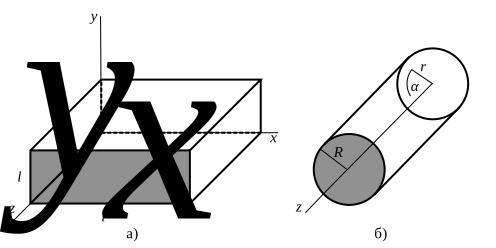
\includegraphics[width = \textwidth]{images/pdf/wave}
		a) прямоугольный волновод;
		б) цилиндрический волновод;
		\caption{Прямоугольный и цилиндрический волноводы}
		\label{figw}
	\end{figure}
	
	Волноводы могут быть изогнутыми, заполненными диэлектриком и вообще любым материалом иметь произвольную переменную форму сечения. Наиболее простой случай~--- волновод, представляющий собой цилиндрическую поверхность с произвольным сечением в основании. Если в основании прямоугольник, то волновод прямоугольный, круг~--- цилиндрический.
	
	\section{Волноводные уравнения}
	
	Рассмотрим волновод произвольного сечения. Два орта перпендикулярных к оси $z$ обозначим $\ort{n}$, $\ort{\tau}$. Поля пропорциональны $\exp i(\omega t - \beta z)$. Операция ротора при таких обозначениях:
	\begin{equation*}
		\rot \vec{E} = 
		\matrixrotr{v}{\tau}{n}{z}{E_\tau}{E_n}{E_z} =
		\matrixt{v}{\ort{\tau} & \ort{n} & \ort{z} \\ \df{\tau} & \df{n} & -i\beta \\ E_\tau & E_n & E_z}
	\end{equation*}
	поэтому уравнения Максвелла для полых волноводов примут вид
	
	\parbox{0.5\textwidth}{
		\begin{align*}
		& \dff{E_z}{n} + i \beta E_n = - i \omega B_\tau \\
		& - \dff{E_z}{\tau} - i \beta E_\tau = - i \omega B_n \\
		& \dff{E_n}{\tau} - \dff{E_\tau}{n} = - i \omega B_z \\
		& \dff{E_n}{n} + \dff{E_\tau}{\tau} - i \beta E_z = 0
		\end{align*}
	}\parbox{0.5\textwidth}{
		\begin{align*}
		& \dff{B_z}{n} + i \beta B_n = i \frac{\omega}{c^2} E_\tau \\
		& - \dff{B_z}{\tau} - i \beta B_\tau = i \frac{\omega}{c^2} E_n \\
		& \dff{B_n}{\tau} - \dff{B_\tau}{n} = i \frac{\omega}{c^2} E_z \\
		& \dff{B_n}{n} + \dff{B_\tau}{\tau} - i \beta B_z = 0
		\end{align*}
	}
	Получим отсюда две подсистемы:
	
	\parbox{0.5\textwidth}{
		\begin{align*}
		& \dff{E_z}{n} = - i \beta E_n - i \omega B_\tau \\
		& - \dff{B_z}{\tau} = i \frac{\omega}{c^2} E_n + i \beta B_\tau
		\end{align*}
	}\parbox{0.5\textwidth}{
		\begin{align*}
		& \dff{B_z}{n} = i \frac{\omega}{c^2} E_\tau - i \beta B_n\\
		& - \dff{E_z}{\tau} = i \beta E_\tau - i \omega B_n
		\end{align*}
	}
	Отсюда следует, что поперечные компоненты поля выражаются через продольные компоненты, поэтому достаточно найти продольные компоненты, чтобы решить задачу. Соотношения для поперечных компонент:
	\begin{align*}
		& {E}_\tau = - i \frac{1}{\gamma^2}\left(\beta\dff{E_z}{\tau} + \omega \dff{B_z}{n}\right) \\
		& {E}_n = - i \frac{1}{\gamma^2}\left(\beta\dff{E_z}{n} - \omega \dff{B_z}{\tau}\right) \\
		& {B}_\tau = i \frac{1}{\gamma^2}\left(\frac{\omega}{c^2} \dff{E_z}{n} - \beta\dff{B_z}{\tau}\right) \\
		& {B}_n = - i \frac{1}{\gamma^2}\left(\frac{\omega}{c^2}\dff{E_z}{\tau} + \beta \dff{B_z}{n}\right)
	\end{align*}
	где обозначено $\gamma^2 = \omega^2/c^2 - \beta^2$, $\gamma$~--- поперечное волновое число. Оставшиеся 4 уравнения Максвелла сводятся к двум уравнениям Гельмгольца простой подстановкой только что полученных соотношений для поперечных компонент:
	\begin{align*}
		& \dfs{E_z}{\tau} + \dfs{E_z}{n} + \gamma^2 E_z = 0 \\
		& \dfs{B_z}{\tau} + \dfs{B_z}{n} + \gamma^2 B_z = 0
	\end{align*}
	Эти уравнения и определяют совместно с соотношениями для поперечных компонент поле в волноводе.
	
	\section{Прямоугольный волновод}
	
	В случае прямоугольного волновода $\partial \tau = \partial x$, $\partial n = \partial y$. Уравнения Гельмгольца:
	\begin{align*}
		& \dfs{E_z}{x} + \dfs{E_z}{y} + \gamma^2 E_z = 0 \\
		& \dfs{B_z}{x} + \dfs{B_z}{y} + \gamma^2 B_z = 0
	\end{align*}
	Будем их решать методом разделения переменных. Примем для начала, что $B_z=0$.  В результате для $E_z$:
	\begin{align*}
		& E_z = (K \sin \gamma_x x + L \cos \gamma_x x) (M \sin \gamma_y y + N \cos \gamma_y y) e^{i (\omega t - \beta z)}
	\end{align*}
	Здесь $\gamma_x$, $\gamma_y$ --- пока неизвестные переменные, которые можно найти из граничных условий.
	
	\chapter{Принцип наименьшего действия}
		
	\section{Свободная релятивистская частица}
	
	Принцип наименьшего действия формулируется всегда таким образом, чтобы действие было инвариантно относительно любых преобразований, и выражает собой тот факт, что движение объектов и тел не зависит от того как наблюдатель движется относительно них или зависит настолько слабо, что этим воздействием можно пренебречь.
	
	Инвариантом относительно преобразований Лоренца (в ОТО вообще относительно произвольных преобразований координат и времени) является интервал:
	\begin{equation*}
		ds^2 = c^2 dt^2 - dx^2 - dy^2 - dz^2 = g_{ij} dx^i dx^j = dx^i dx_i.
	\end{equation*}
	По этой причине действие следует искать в форме:
	\begin{equation*}
		S(1, 2) = \int\limits_{1}^{2} A\, ds,
	\end{equation*}
	где $A$ --- константа, такая, что в нерелятивистском случае подынтегральное выражение переходит в функцию Лагранжа с точностью до константы и множителя $dt$:
	\begin{equation*}
		A ds = A c \sqrt{1 - \frac{v^2}{c^2}} dt = A c \left( 1 - \frac{1}{2} \frac{v^2}{c^2} + \ldots \right) dt,
	\end{equation*}
	сравнивая с нерелятивистским выражением
	\begin{equation*}
		\frac{mv^2}{2} dt,
	\end{equation*}
	получаем 
	\begin{equation*}
		A = - mc.
	\end{equation*}
	Действие для свободной релятивистской частицы:
	\begin{equation*}
		S(1, 2) = -\int\limits_{1}^{2} mc\, ds.
	\end{equation*}
	
	Вариация от действия по $x^i$ будет связана с вариацией от интервала:
	\begin{equation*}
		\delta\, ds^2 = 2 ds\, \delta\, ds  = d\, \delta x^i dx_i + d\, \delta x_i dx^i = 2 d\, \delta x^i dx_i.
	\end{equation*}
	Отсюда:
	\begin{equation*}
		\delta\, ds = u_i d\, \delta x^i = d (u_i \delta x^i) - du_i \delta x^i = - du_i \delta x^i.
	\end{equation*}
	Здесь отброшен полный дифференциал, который после интегрирования будет давать 0. Далее также будут отбрасываться полные дифференциалы. 
	
	Уравнения движения свободной релятивистской частицы:
	\begin{equation*}
		mc \Dff{u_i}{s} = 0.
	\end{equation*}
	То есть свободная релятивистская частица движется с постоянной четырёхскоростью.
	
	\section{Инварианты взаимодействия частицы с векторным полем и их вариации}
	
	Векторное поле $A_i$ действует на частицу. У частицы есть три характеристики $x_i$ --- координата, $u_i$ --- четырёхскорость, $w_i$ --- четырёхускорение. С векторным полем $A_i$ три эти характеристики дают инварианты:
	\begin{gather*}
		A_i(x^j) x^i, A_i(x^j) u^i, A_i(x^j) w^i,
	\end{gather*}
	но последний инвариант при вариации даст уравнения выше второго порядка и по этой причине его следует отбросить, так как мы полагаем, что движение частицы полностью определяется начальной скоростью и положением частицы, а первый инвариант нарушает представления об однородности пространства. В дополнение к этим инвариантам идут инварианты поля, но пока ограничимся инвариантом
	\begin{align*}
		& S_1 = A_i u^i.
	\end{align*}
	Действие будет в виде:
	\begin{equation*}
		S(1, 2) = \int\limits_{1}^{2} f(S_1) ds,
	\end{equation*}
	где $f(S_1)$ --- пока неизвестная функция. Вариация от действия сведётся к вариации от инварианта. Найдём её:
	\begin{gather*}
		\delta S_1 = 
		u^k \dff{A_k}{x^i} \delta x^i + A_i \Dff{\delta x^i}{s} = 
		u^k \dff{A_k}{x^i} \delta x^i + \Dff{A_i \delta x^i}{s} - \Dff{A_i}{s} \delta x^i = \\ =
		u^k \left( \dff{A_k}{x^i} - \dff{A_i}{x^k} \right) \delta x^i = F_{ik} u^k.
	\end{gather*}
	Из силы Лоренца следует, что 
	\[
		\dff{f(S_1)}{S_1} = q.
	\]
	Действие для частицы в поле имеет вид:
	\[
		\int - mc\, ds + q A_i\, dx^i.
	\]
	Уравнения движения в четырёхмерном виде:
	\[
		mc \Dff{u_i}{s} = F_{ik} u^k.
	\]
	
	\section{Инварианты поля и уравнения для полей}
	
	 Инварианты поля такие, что при вариации по полю продолжает работать принцип суперпозиции, то есть $A_i$ входит в инварианты максимум во второй степени, и такие, что поле полностью определяется своими значениями и производными на границе(то есть уравнения поля должны быть не выше второго порядка, а в инварианты могут входить только производные первого порядка от поля):
	 \begin{gather*}
	 A_i(x^j) A^i(x^k), \dff{A^i}{x^i}, \dff{A^i}{x^j} \dff{A^j}{x^i}.
	 \end{gather*}
	 Второй инвариант при калибровке Лоренца равен нулю. Последний инвариант эквивалентен инвариантам:
	 \[	
	 	F_{ik}F^{ki}, \tilde{F}_{ik} \tilde{F}^{ki}.
	 \]
	 Поле --- протяжённая система, поэтому действие поля должно иметь вид:
	 \[
	 \int\limits_{} f(inv) d^4 x.
	 \]
	 
	 
	
\end{document}